\documentclass{article}
\usepackage[utf8]{inputenc}
\usepackage{geometry}
\usepackage{fancyhdr}
\usepackage{listings}
\usepackage{caption}
\usepackage{graphicx}
\usepackage{xltabular}
\def\code#1{\texttt{#1}}
\setcounter{section}{-1}
\parskip=8pt
\parindent=10pt
\setlength{\headheight}{15.2pt}
\pagestyle{fancy}
\geometry{left=3cm,right=3cm,top=3cm,bottom=3cm}
\usepackage{hyperref}
\begin{document}

\begin{titlepage}
	\begin{center}
	{\scshape\LARGE Wilfrid Laurier University\par}
	{\scshape \LARGE CP465 LEAD Project \par}
	\vspace{1cm}
	{\huge\bfseries News Article Search Engine\par}
	\vspace{1cm}
	{\Large\itshape \raggedleft Anthony Sukadil, 160593610 \newline Celeste Shattuck, 170494820 \newline\par}		
	\vspace{1cm}
	{\large \today\par}
	\end{center}
\end{titlepage}
\rhead{CP465, \today, LEAD Project}
\section{Initial Project Proposal}
\subsection{Project Paradigms}
The project paradigms we’re going to be using are JavaScript/TypeScript (Angular frontend) and a Python backend using Flask. Data processing will be done using Python since it’s very flexible and easy to maintain. Data storage will be in done a table-oriented format (CSV) and other methods such as an inverted index will be stored on disk.
\subsection{Project Theme}
The project theme will be an information retrieval/search engine-based project about news articles called the News Article Search Engine Project. Since news is all around us and we want to find the most intriguing news article to read, we will develop a tool to find relevant documents. Using keywords in a search bar, users can find the most relevant documents using different searching methods and compare their overall efficiency and effectiveness in finding related documents.
\subsection{Resources for Project}
In terms of resources, since this project will not be hosted on any platform, for hardware, we won’t need extra compute power or external providers for the implementation of this project, most of it will be hosted on the local machine. Software wise, we’re only going to be using the programming languages discussed earlier, which again will be on the local machine. \newline \newline
For external literature sources, we will need to look at methods of determining document relevancy such as TF-IDF or Levenshtein distance and the textbook for relevant topics.
\subsection{Project Risks}
\begin{enumerate}
    \item Not being able to fully optimize the data processing techniques
    \item Not being able to connect with other group members to communicate issues
    \item Unfamiliarity with methods of determining document relevancy
    \item Using programming paradigms that are not as comfortable, leading to less efficient code
\end{enumerate}
\subsection{Data used for Project}
The data we’re going to be using is from Kaggle (\url{https://www.kaggle.com/snapcrack/all-the-news}), which is dataset consisting of news articles from 15 American publications. The data model will fall accordingly to the dataset and any other relevant models used for determining document relevancy.
\subsection{Project languages}

We’re going to have an Angular powered frontend with a Python powered backend. Angular has a nice feature called Pipes which are useful in filtering results in an elastic fashion. Python is chosen for the backend since text processing in Python is much easier and it is widely used within the machine learning community. Flask will be used to serve endpoints which the frontend can request for results, so for example queries like 
\verb|/document?query=business&pub_date=gte2018| can be processed in their respective endpoints. This will require us to build the tables first using Python which can take some time, but we will 
store models on disk for quicker reference.
\subsection{CVS structure}
The CVS structure is as follows:\newline
ID, Title, Publication, Author, Date, Year, Month, URL, Content 
\subsection{Project Timeline}
\begin{center}
    \begin{tabular}{|m{5cm}|m{5cm}|m{5cm}|}
    \hline
    Task & Steps to Solve & Milestone step achieves     \\ \hline
    Understand our dataset & Look at the columns and what they represent and is there anything that’s missing that could be important before processing    & Data assessment and validity               \\ \hline
    Layout project tools for easier development       & Discuss with team members about committing code to the project such as Trello, GitHub, etc.     & Project management and guidelines               \\ \hline
    Research methods for information retrieval/text processing      & Find articles, papers, and read the textbook talking about information retrieval techniques and methods of processing textual data such as TF-IDF    & Method of processing our dataset    \\ \hline
    Implement the research found into the backend      & Using Python, implement the algorithms discussed in the previous step into file storage (to avoid re-computation)  & Finished data compilation for querying  \\ \hline
    Setup relevant endpoints      & Using Flask, setup respective endpoints for the frontend to query & Backend endpoints for frontend \\ \hline
    Design the frontend layout  & Use HTML and CSS to design a basic layout for querying and displaying results & A U.I. that is interactable \\ \hline
    Test all components together     & Act as a user who uses the application for intuitiveness, ease of use, and speed       & Fast, reliable, and intuitive       \\ \hline
    \end{tabular}
\end{center}

\section{Project submission}
\subsection{Deviation from initial proposal}
Our main deviation from the initial project was more of an addition to the original proposed scope than it was a deviation per sey.
During the project RIP which had taken place on March 20th 2021, we had concerns that we were not doing enough.
It was then that we decided that we would add a secondary search method with a different model to the project. As a result we used K-means clustering and bag of words model to implement our secondary search method.
The original project paradigm mentioned the use of an inverted index.
The inverted index mentioned was not implemented, but instead was changed into a secondary index instead.
In addition to this, a way to compare the two were also added by timing how long it had taken each method to return the results and displaying this number to the user.

\subsection{Back-end Design}
The back end is divided into multiple sections. \newline
The data we are working with is found in /server/data folder. \newline
Our article fetcher relies on transferring this data to models so that they are preprocessed before the user searches, and has a faster result than processing the articles into models every time a new query is made, these models are found in /server/data/models folder.\newline
Application.py is then used as way for the front end components to connect to the back end, make queries and retrieve the articles to be put into the corresponding components for display by the results component.
\subsection{Supported Queries}
\begin{enumerate}
    \item The user can select a keyword to search by. If the user enters a keyword such as "Trump" as seen in Figure 3 below, a number amount articles that are related in a specified with Trump are returned.
    \item The user can choose how they would like the returned articles to be searched. The options included are Article Content and Article Title, depending on which the user decides to use has a large impact on what results are returned to the user in both search methods.
    \item The user can select how many results they wish to be returned to them. When n is the number the user has selected, n TF-IDF articles are returned, and n secondary indexing articles are returned for a total of 2n articles returned to the user.
\end{enumerate}

\subsection{Front-end design}
\subsubsection{Initial Screen}
When a user first launches the web app on their local host they are greeted with this screen.
The screen is split in between two sides for comparing the speeds of retrieval when the user makes a query.
\begin{figure}[htp]
    \centering
    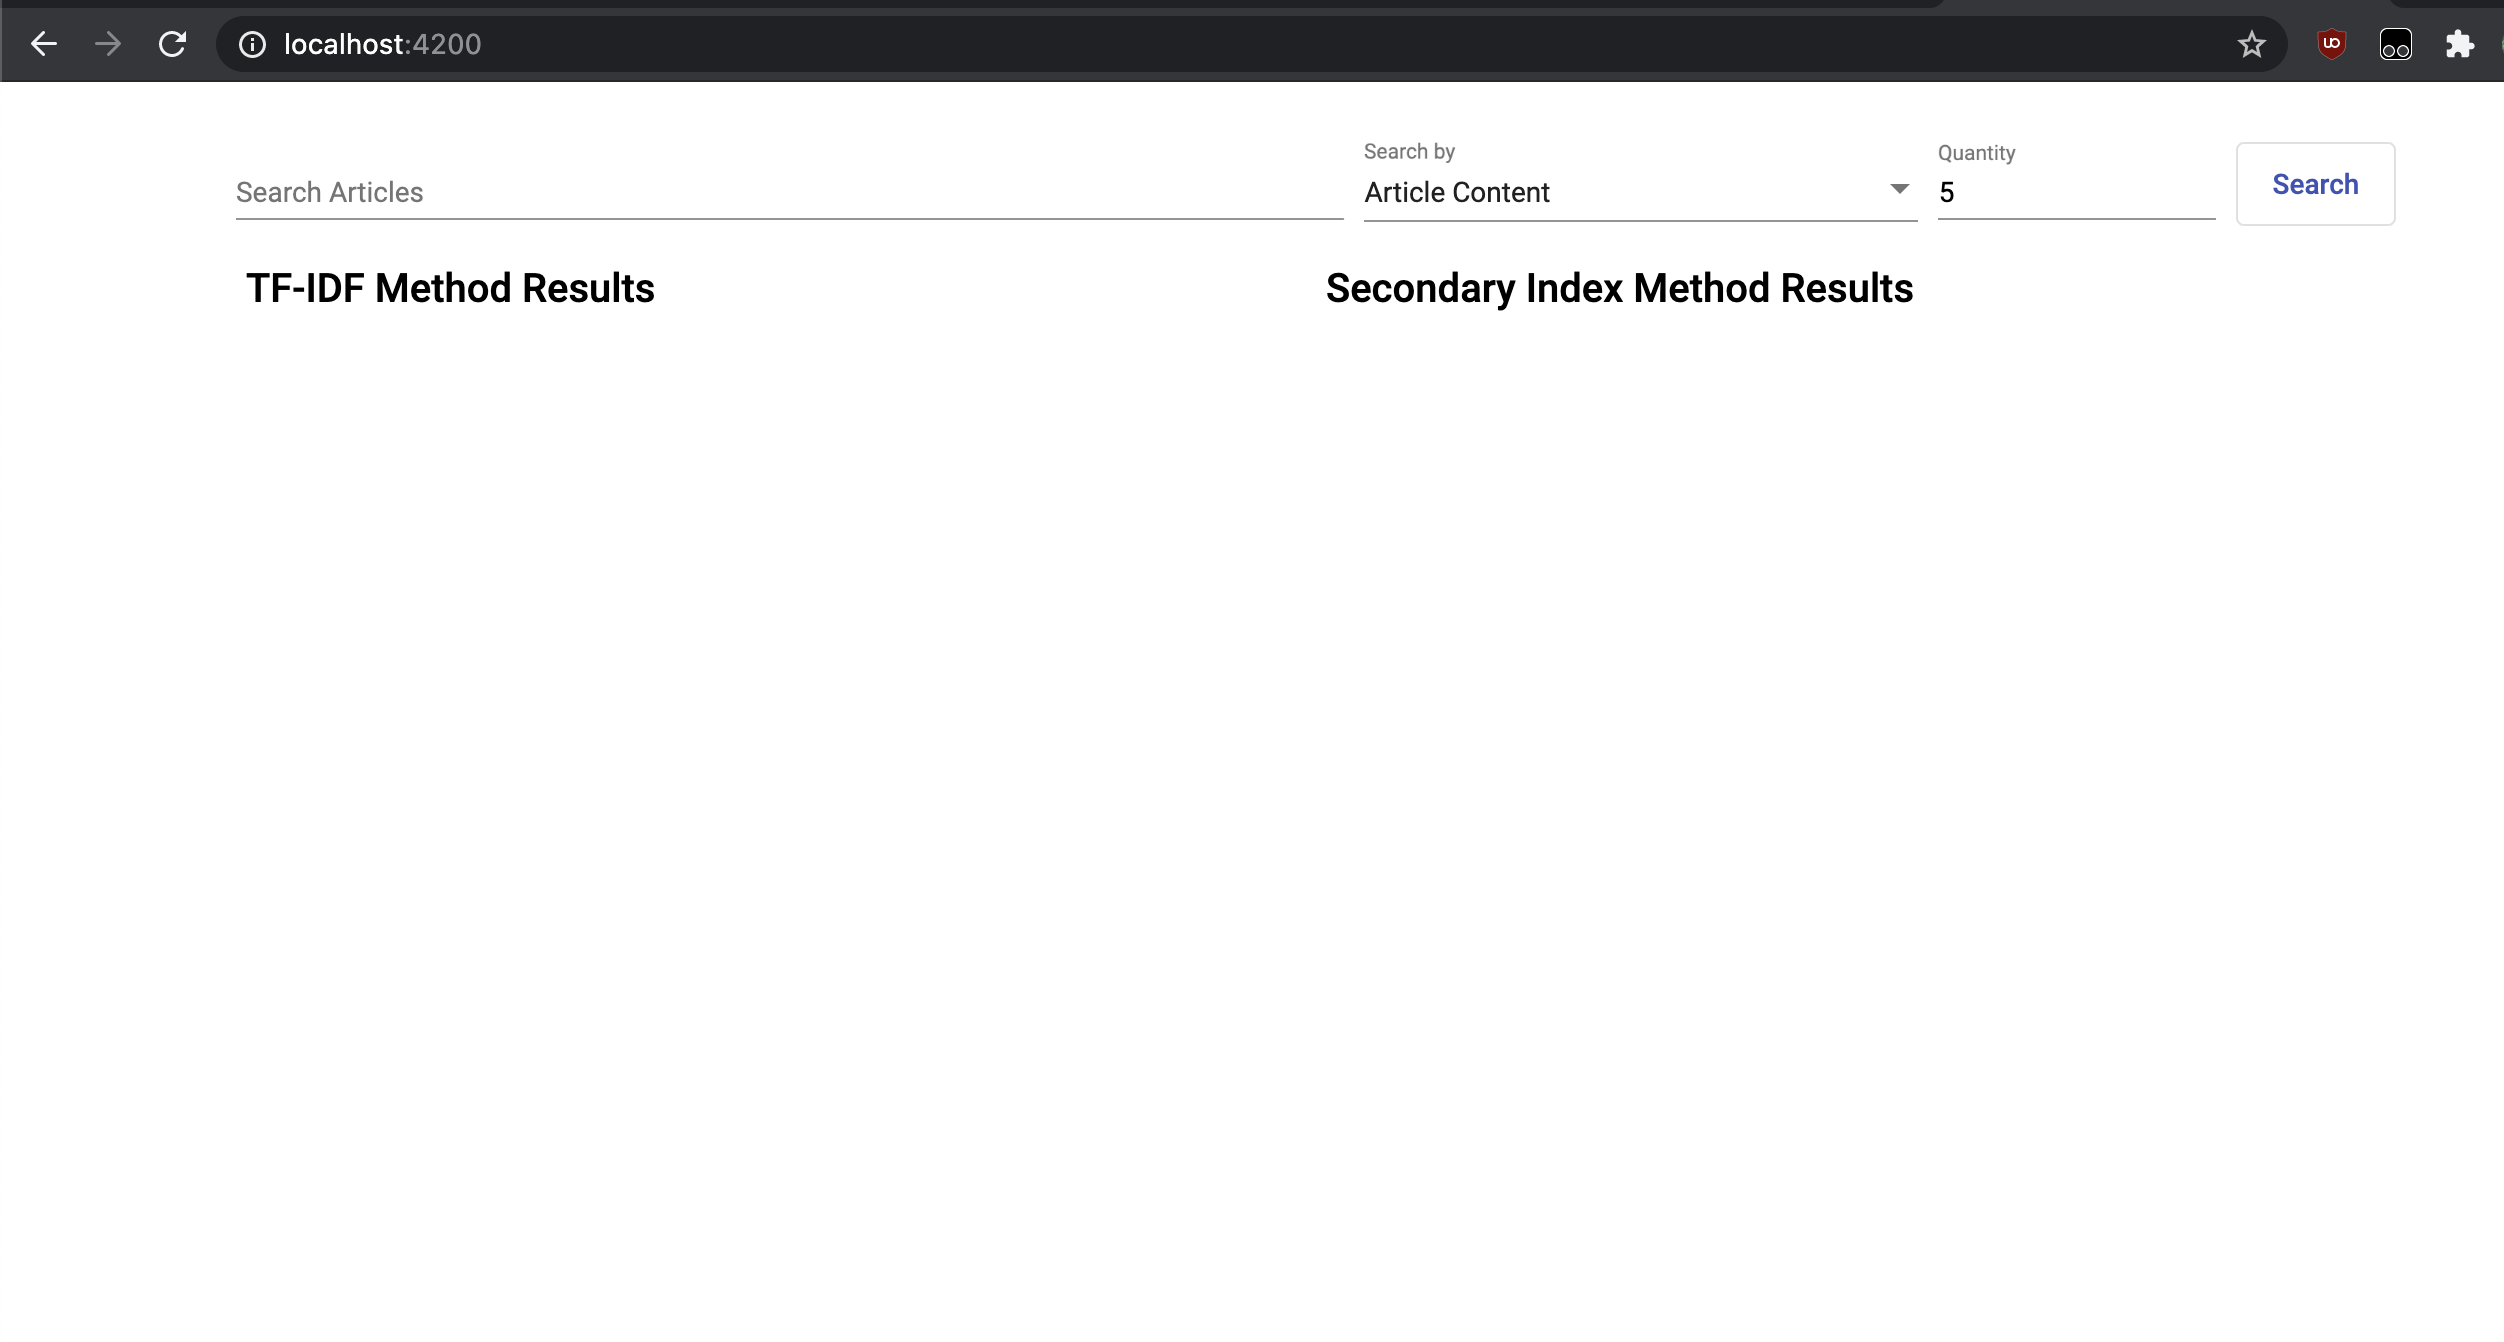
\includegraphics[width=15cm]{InitialScreen.png}
    \caption{Initial Screen on launch}
\end{figure}
\subsubsection{Search Options}
Before making a new search, the user has the option to select to "Search by Article Content" or to select "Search by Article Title". These options change the results that are returned. Searching by Article Title uses the Article Title alone against the search query to return a result, likewise if the user selects to search by Article Content, the title of the article will be ignored and results will be based on strictly the content when matched with the word or words the user searches by.
\begin{figure}[htp]
    \centering
    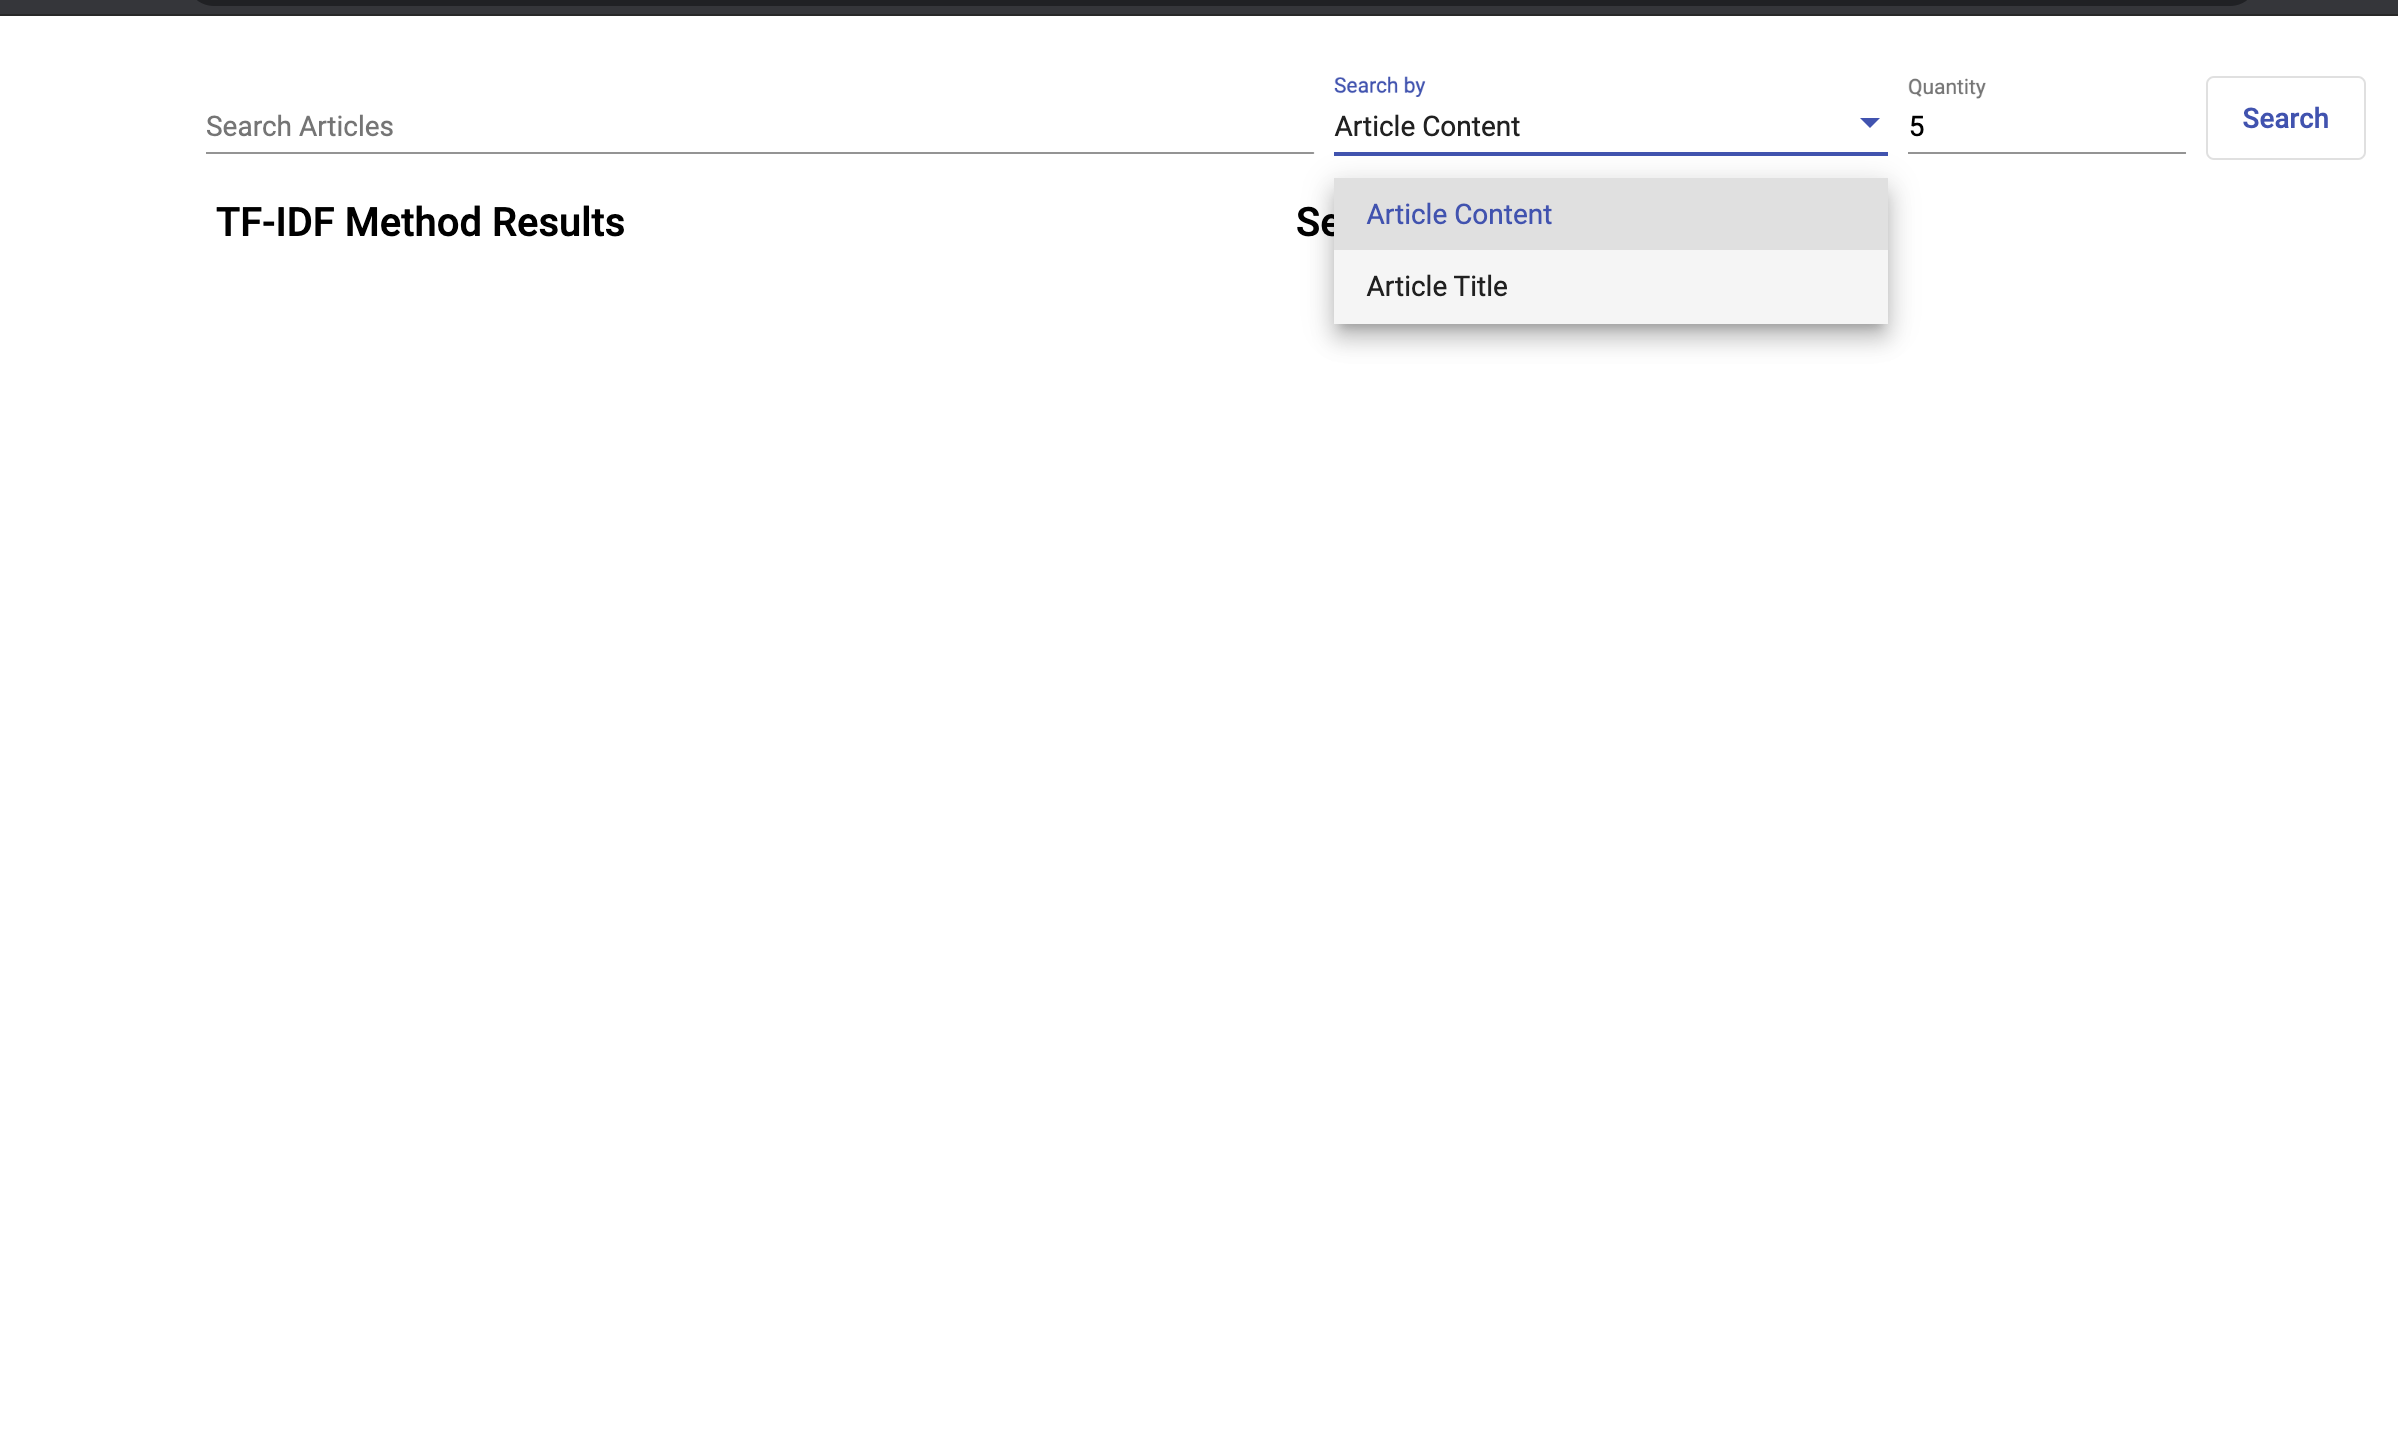
\includegraphics[width=15cm]{SearchByDrop.png}
    \caption{Search options}
\end{figure}
\subsubsection{Initial Results}
When the user makes a query, it is divided into two parts. Documents returned by TF-IDF or term frequency–inverse document frequency, the other search result is the secondary index method. The secondary index method was made by using the Bag of Words model, followed by using K-means to cluster this data. Both result methods also show to the user the time it takes to carry out the result using the specific method.
\begin{figure}[htp]
    \centering
    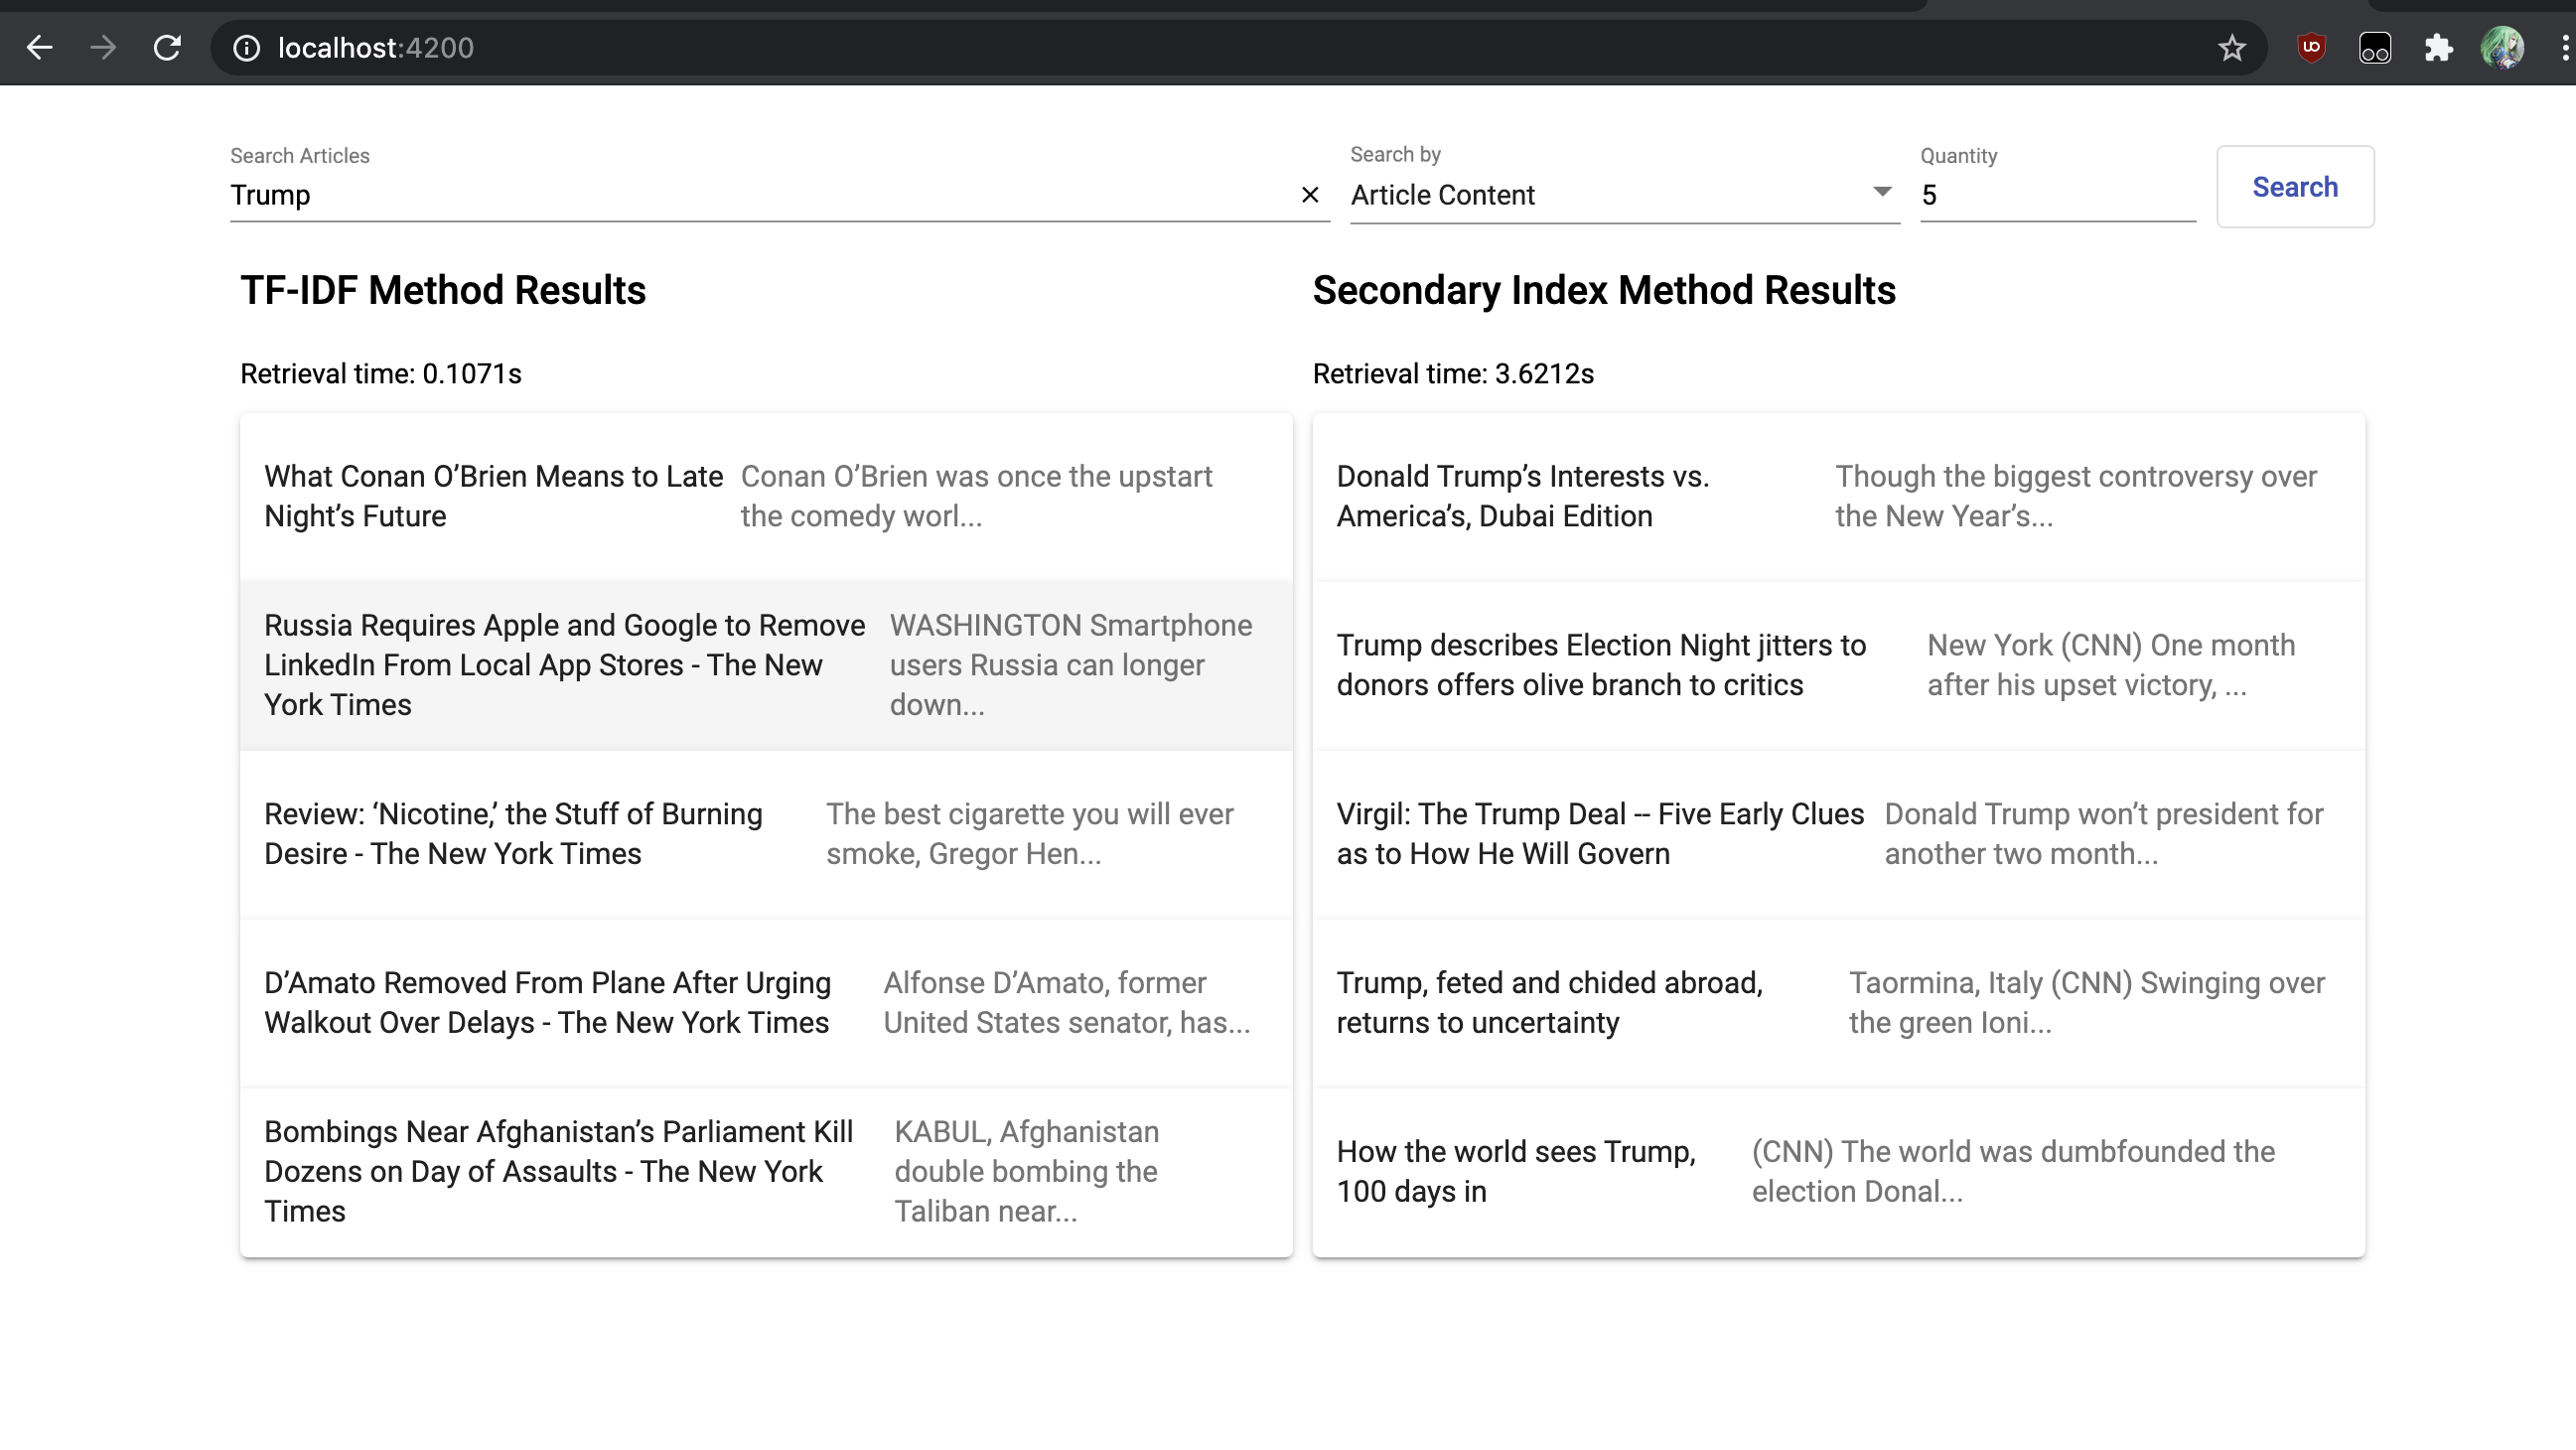
\includegraphics[width=15cm]{Results.png}
    \caption{Results Example}
\end{figure}
\subsubsection{Enhanced Results}
When a user selects a given return article in the results, the full article opens up for the user, allowing the user to read the article that was returned by the search engine
\begin{figure}[htp]
    \centering
    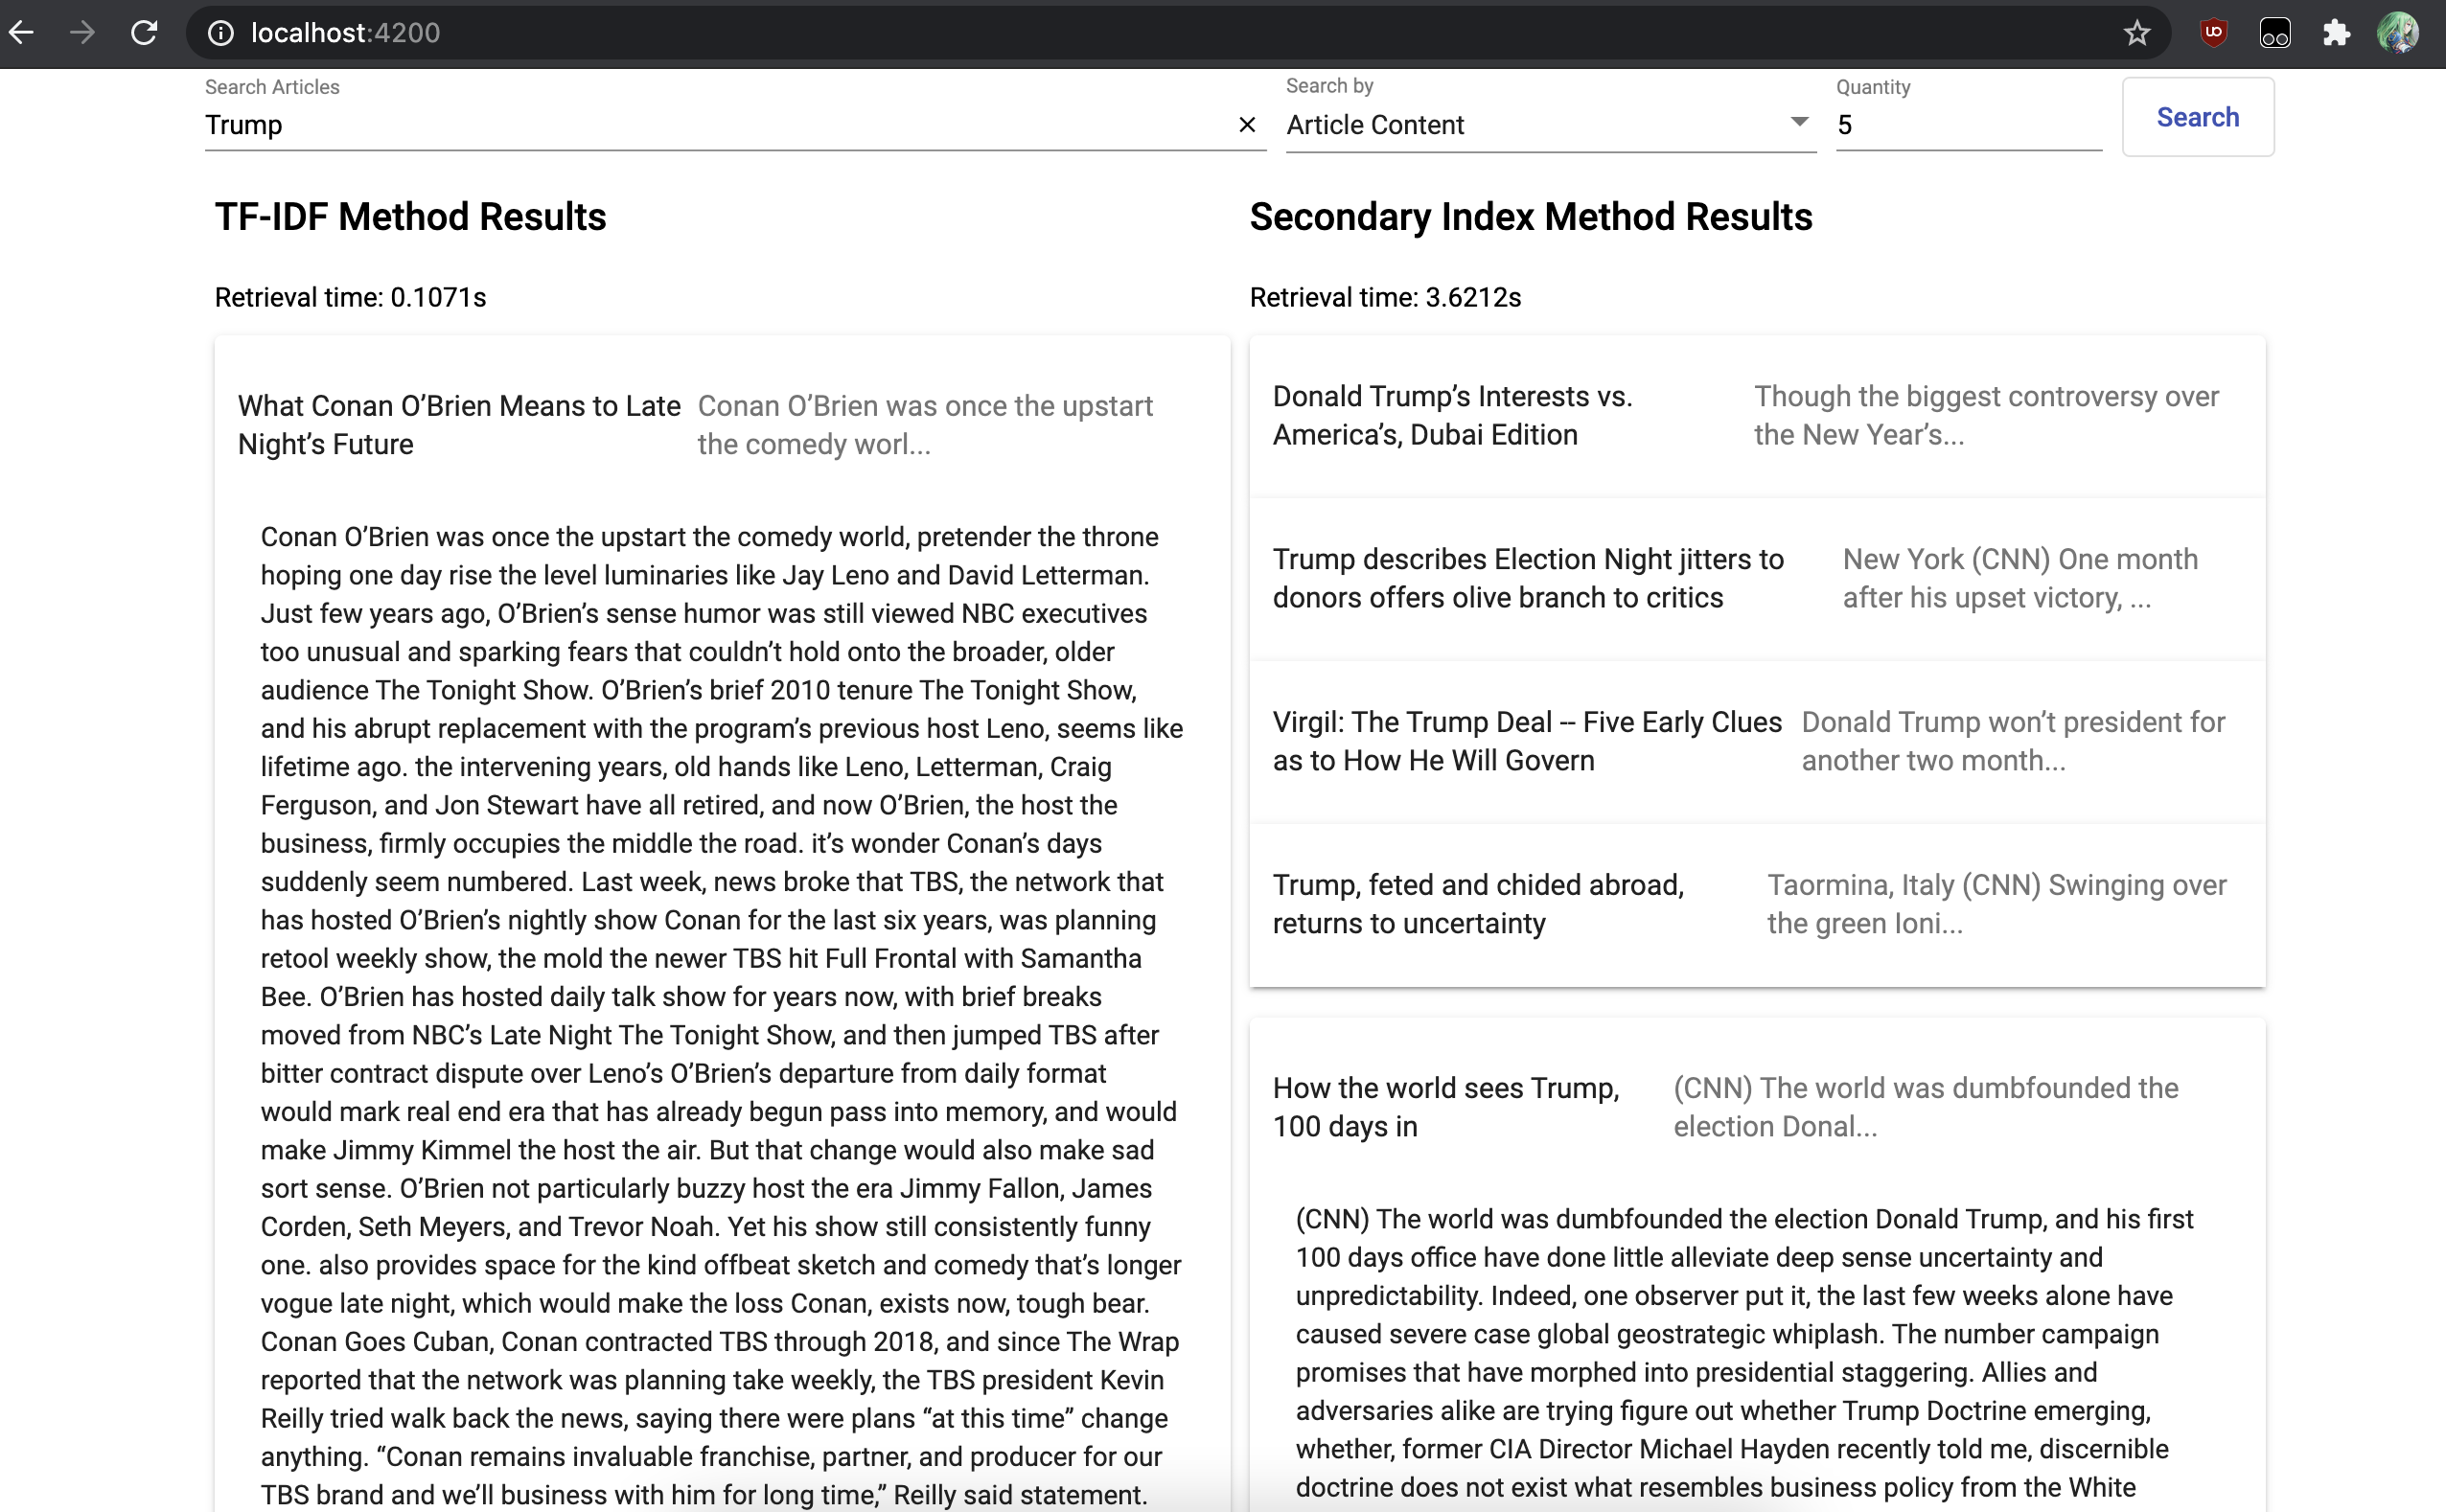
\includegraphics[width=15cm]{ResultsDetail.png}
    \caption{Enhanced Results Example}
\end{figure}
\newpage
\subsection{Project functionalities}
The project successfully acts like a search engine and returns articles to the user based on their keyword search, the user's between returning articles based on the content, or the title of the article.
The steps that the project take are as follows.
\begin{enumerate}
    \item The user enters a keyword in the search bar, selects to search by Article Contents, or Article Title, and selects how many articles they would like to be retrieved under each model.
    \item When the user clicks search, an event is called, and a query function begins, this checks what the user has inputted, and goes to make two queries to the back end where the data is stored. This is called in Application.py
    \item Application.py reads these queries, and uses the corresponding TF-IDF (either content or title) models and the corresponding secondary index models to retrieve and store these article objects in a list.
    \item The two lists are then returned in a readable format, with the amount of time it had taken for the query to be fulfilled under each search method to the app component in the frontend.
    \item The app component then sends the lists to the results component to be placed into the panels as seen in Figure 3, and is then visible to the user as such.
\end{enumerate}
\section{Conclusion}
Throughout the project team members learned many things such as learning more about how basic search engines work, and what kinds of methods are used in them, as well as learning methods that do not work so well when it is faster results that we want.
We learned that the TF-IDF method is more efficient to return to the user documents at a higher speed.
It was also found that although slower, that the secondary search method returned articles with more mentions of the searched word.
An example is when one searches for Trump as seen in Figure 3. The top result in TF-IDF has 0 (zero) mentions of Trump, however the secondary search method top result has 210 mentions of Trump in the article.
This is just an example however, and does not apply to all queries, such as when the user searches "Clinton" both methods have the same top result, and have some matching results in a different order.
Though it was somewhat expected to have completely different results, it was interesting to see how different these results would actually be.
Overall, we learned how important it is to use different methods in a search engine, so that when returning documents to a user, they receive the most relevant results across the board to their query.

\section{Member Contributions}
\begin{enumerate}
    \item Anthony: xx\%
    \item Celeste: xx\%
\end{enumerate}

\end{document}
